\section{Контрольные вопросы}

\textbf{
    1. Что такое единичная ступенчатая функция
    $ \delta_{1}(t), \delta_{1}(t-\tau) $ ?
}

Единичная ступенчатая функция $ \delta_{1}(t) $ 
определяется как:

\begin{equation}\label{eq:esf}
\delta_{1}(t) = 
\begin{cases}
    0, & t < 0\\
    1, & t \ge 0
\end{cases}
\end{equation}

Функцию $ \delta_{1}(t-\tau) $  мы получаем из ЕСФ путем смещения вправо на величину $ -\tau $, она называется запаздывающей единичной ступенчатой функцией.

\begin{equation}\label{eq:esft}
\delta_{1}(t-\tau) = 
\begin{cases}
0, & t < \tau\\
1, & t \ge \tau
\end{cases}
\end{equation} 

\textbf{
    2. Нарисуйте графики функций 
    $ f_{1}(t) = 2 e^{-t} \delta_{1}(t) $ и 
    $ f_{2}(t) = 2 e^{-t-\tau} \delta_{1} (t-\tau) $
}

\begin{figure}[H]
    \centering
    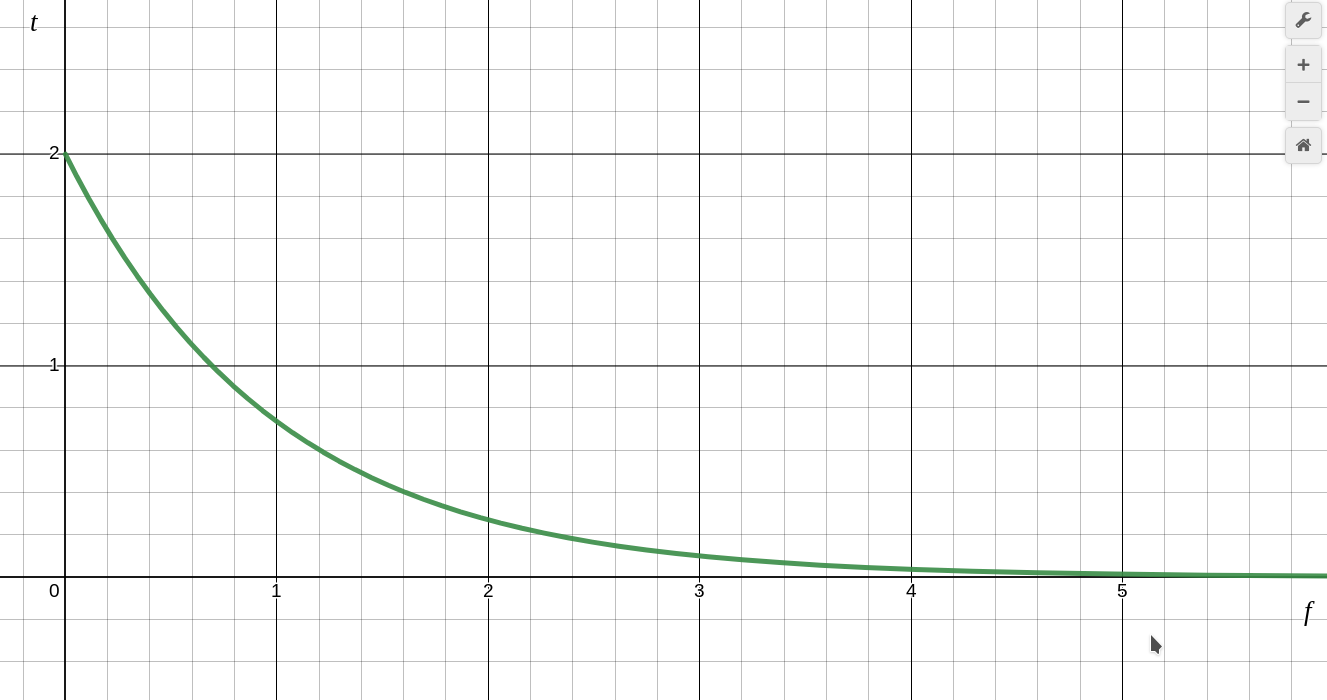
\includegraphics[width=0.7\linewidth]{photo/q2_1}
    \caption{График $ f_{1}(t) = 2 e^{-t} \delta_{1}(t) $}
    \label{fig:q2_1}
\end{figure}

\begin{figure}[H]
    \centering
    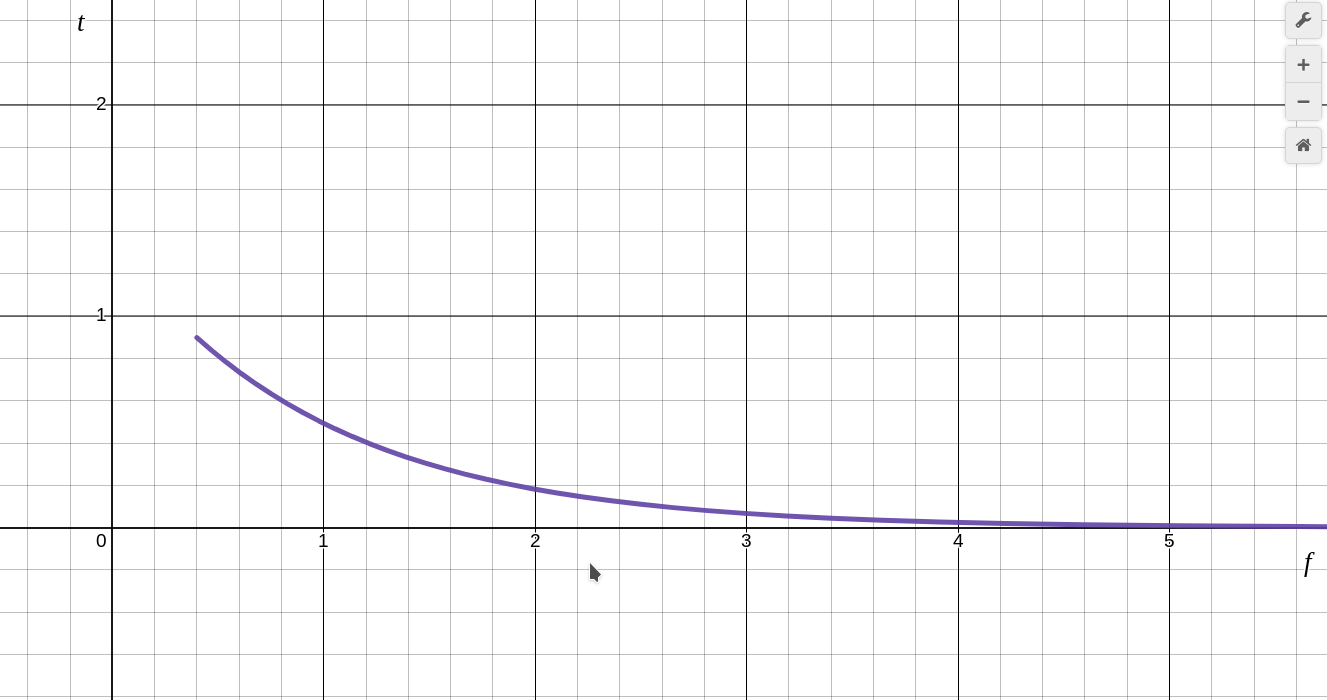
\includegraphics[width=0.7\linewidth]{photo/q2_2}
    \caption{График $ f_{2}(t) = 2 e^{-t-\tau} \delta_{1} (t-\tau) $ ($ \tau = 0.4 $)}
    \label{fig:q2_2}
\end{figure}

\textbf{
    3. Определите $ f(0^+) $ и $ f(1^+) $, если \\
    $ f(t) = 
    4 e^{- t    } \cos(2 \pi t    ) \delta_1(t) -
    4 e^{- (t-1)} \cos(2 \pi (t-1)) \delta_1(t-\pi)
    $
}\\

$ f(0^+) = 
4 e^{0} \cos( 2 \pi 0) \delta_{1}(0   ) - 
4 e^{1} \cos(-2 \pi  ) \delta_{1}(-\pi) = 
4 \cdot 1 \cdot 1 \cdot 1 - 
4 \cdot e \cdot 1 \cdot 0 = 
4
$

$ f(1^+) = 
4 e^{-1    } \cos(2  \pi  ) \delta_{1}(1)    - 
4 e^{-(1-1)} \cos(-2 \pi 0) \delta_{1}(1-pi) =
\dfrac{4}{e} \cdot 1 \cdot 1 - 
4 \cdot 1 \cdot 1 \cdot 0 = 
\dfrac{4}{e} 
$

\textbf{
    4. Что называется переходной характеристикой цепи?
}

Переходной характеристикой цепи $ h_{1}(t) $ называется реакция цепи при ее нулевых независимых начальных условиях на единственное в цепи воздействие в виде единичной ступенчатой функции $ \delta_{1}(t) $

\textbf{
    5. Какой вид имеет вынужденная составляющая $ h_{1}(t) $ ?
}

При постоянной воздействии вынужденная составляющая переходной характеристики цепи образует константу $ h_{1св}(t) = const $ 

\textbf{
    6. Перечислите способы определения $ h_{1}(t) $.
}

Определить переходную характеристику цепи 
$ h_{1}(t) $ можно по уравнениям состояния, 
приведенными в п. \ref{sec:analysis} 
настоящей курсовой работы
(\ref{eq:state}).

При нулевых независимых начальных условиях, 
переходную характеристику цепи 
можно найти как 
оригинал изображения-передаточной функции 
$ h_{1}(t) = \mathcal{L}^{-1}[H(s)] $

\textbf{
    7. Характеристическое уравнение цепи 
    $ p^{2} + 6p + 8 = 0 $. 
    Какой вид имеет свободная составляющая $ h_{1}(t) $?
    Оцените $ t_{ПП} $.
}

Корни характеристического уравнения:

$$ p_{1,2} = \dfrac{-6 \pm 2}{2} = -2, -4 $$

Значит, $ h_{1}(t) $:

$$ 
h_{1}(t) = (
    A_{1} \, e^{-2t} + 
    A_{2} \, t \, e^{-4t} + 
    const
) \, \delta_{1}(t) $$

Тогда, $ t_{ПП} $:

$$ t_{ПП} = \dfrac{3}{|s|_{\min}} = \dfrac{3}{2} = 1.5 с $$

\textbf{
    8. Характеристическое уравнение цепи 
    $ p^{2} + 10p + 25 = 0 $. 
    Какой вид имеет свободная составляющая $ h_{1}(t) $?
    Оцените $ t_{ПП} $.
}

Корни характеристического уравнения:

$$ p_{1,2} = \dfrac{-10}{2} = -5 $$

Значит, $ h_{1}(t) $:

$$ 
h_{1}(t) = (
A_{1} \, e^{-5t} + 
A_{2} \, t \, e^{-5t} + 
const
) \, \delta_{1}(t) $$

Тогда, $ t_{ПП} $:

$$ t_{ПП} = \dfrac{3}{|s|_{\min}} = \dfrac{3}{5} = 0.6 с $$

\textbf{
    Как определить значения 
    $ h_{1}(0+) $  и  $ h_{1}(\infty) $ 
    в цепи непосредственно по схеме, 
    без вычисления $ h_{1}(t) $?
}

Для этого нужно построить схемы замещения:
 
$$ t \rightarrow 0      \; (L = XX, C = К3) $$
$$ t \rightarrow \infty \; (L = К3, C = XX) $$. 

Так, значения 
$ h_{1}(0^+) $  и  $ h_{1}(\infty) $  
будут равны току или напряжению на 
искомых нагрузках:

$$ h_{1}(0+)     = X_{н}(0)      $$
$$ h_{1}(\infty) = X_{н}(\infty) $$

\textbf{
    10. Цепь задана тройками чисел: 
    113 - $ u_1 $; 
    223 - $ R_2 $ = 6; 
    312 - $ R_3 $ = 3; 
    423 - $ L $ = 1. 
    Как определить $ h_{1}(t) $ для $ u_2 $?
}

\begin{figure}[H]
    \centering
    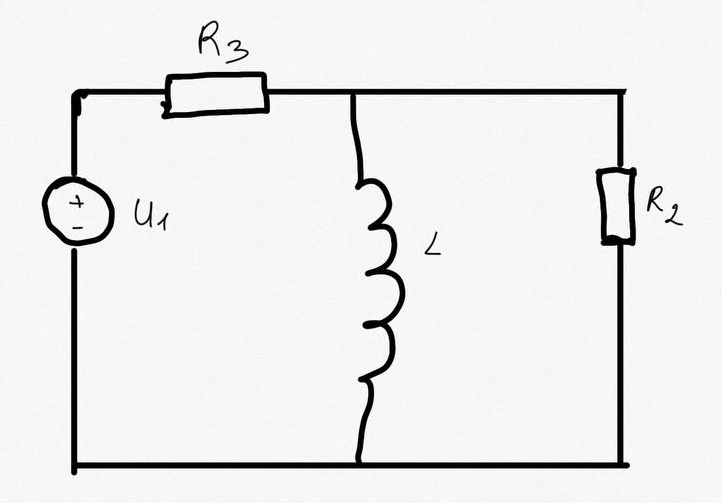
\includegraphics[width=0.7\linewidth]{photo/q10}
    \caption{Цепь}
    \label{fig:q10}
\end{figure}

Найдем напряжение на $ R_2 $:\\

$ u_2(t) = A \, e^{-\frac{t}{\tau}} + U_{2уст.} $\\

По схеме замещения
при $ t \rightarrow \infty $ ($ L = К3 $)
установившееся напряжение будет равно нулю
(параллельно КЗ). 

Постояннная времени $ \tau $:

$ \tau = \dfrac{L}{R_{экв}} = \dfrac{1}{2} $

ЗНУ при $ t = 0^+ $ :

L = ИТ $ t =0^{-} $, отсюда 

$ i_{вх} =  \dfrac{1}{9} $

$ U_{2}(t) = \dfrac{1}{9} \cdot 6 = \dfrac{2}{3} $

Постоянная интегрирования $ A $:

$ U_{2}(0^+) = Ae^{-2t} + U_{2уст} $

$ A = \dfrac{2}{3} $

В итоге, 
$ h_{1}(t) $ для $ u_2 $ будет:

$$ h_{1}(t) = \dfrac{2}{3} \, e^{-2t} $$

\textbf{
    11. Цепь задана тройками чисел: 
    113 - $ u_1 $; 
    223 - $ R_2 $ = 3; 
    312 - $ R_3 $ = 6; 
    423 - С = $ \dfrac{1}{4} $. 
    Как определить $ h_{1}(t) $ для u2?
}

Решим данную задачу операторным методом. 

Сначала определим передаточную функцию 
$ H_{U}(s) $ : 

$ 
U_{2} = 
                  1 \rightarrow U_{C} =
                  1 \rightarrow I_{2} = 
       \dfrac{1}{3} \rightarrow I_{C} = 
       \dfrac{s}{4} \rightarrow I_{3} = 
\dfrac{4 + 3S}{12S} \rightarrow U_{3} =\\\\=
  \dfrac{4 + 3S}{2} \rightarrow U_{1} = \dfrac{6 + 3S}{2} 
$\\

$ H_{U}(s) = \dfrac{2}{6 + 3S} ,\; s = -2 $\\

$ 
h_{1}(t) = 
\lag{\dfrac{\dfrac{2}{3}}{s(s + 2)}} = 
\dfrac{A}{s + 2} + \dfrac{B}{s}
$\\

$ 
A = 
\mylim[s]{-2}{(s+2)\dfrac{\dfrac{2}{3}}{s(s + 2)}} =
-\dfrac{1}{3}
$\\

$ 
B = 
\mylim[s]{0}{s\dfrac{\dfrac{2}{3}}{s(s + 2)}} =
\dfrac{1}{3}
$

$$ h_{1}(t) = -\dfrac{1}{3} e^{-2t} + \dfrac{1}{3} $$

\textbf{
    12. Цепь задана тройками чисел: 
    115 - $ u_1 $; 
    213 - $ R_2 = 4 $; 
    325 - $ R_3 = 4 $; 
    445 - $ R_4 = 4 $; 
    512 - L; 
    634 - C. 
    Как определить 
    $ h_{1}(0^+) $ и $ h_{1}(\infty) $ для $ u_4 $?
}

\begin{figure}[H]
    \centering
    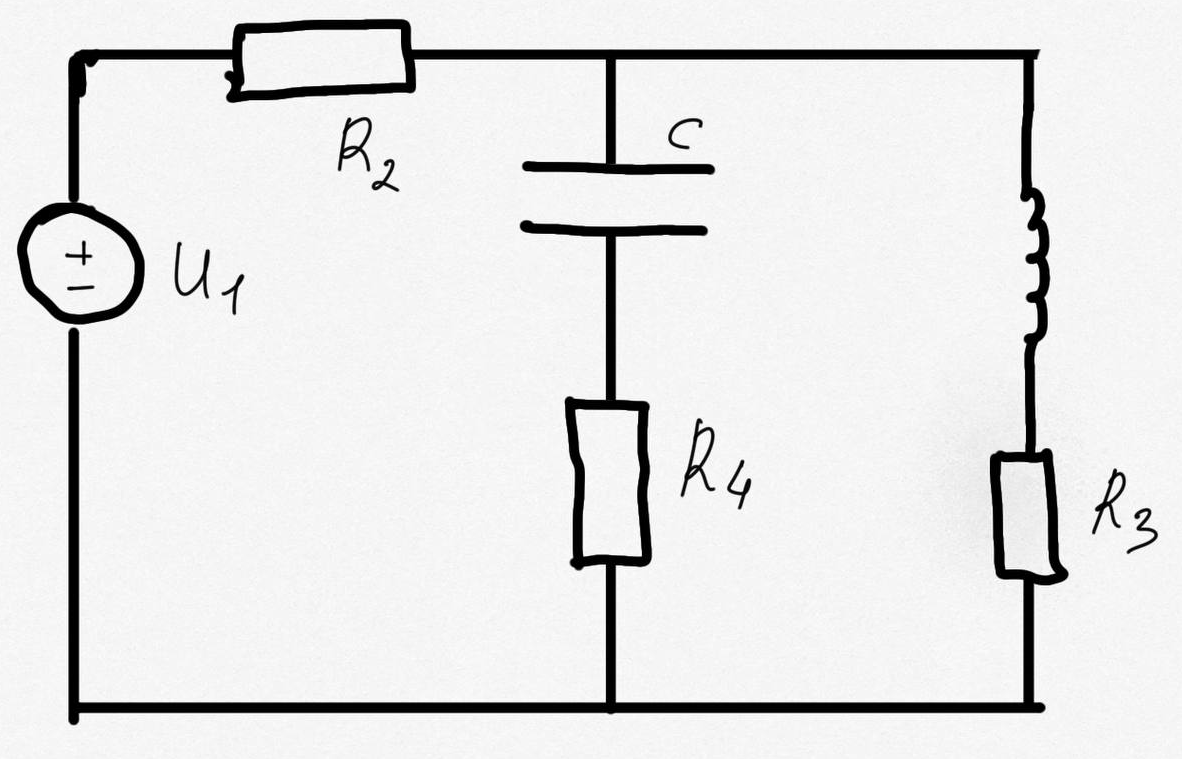
\includegraphics[width=0.7\linewidth]{photo/q12}
    \caption{Цепь}
    \label{fig:q12}
\end{figure}

При $ t = 0 $: $ L = XX, С = К3 $ 

$$ h_{1}(0+) = i_{вх} \cdot R_{4} = 0.5 \, u_1 $$

При $ t \rightarrow \infty$: $ L = КЗ, С = ХХ $  
 
$$ h_{1}(\infty) = 0 $$

\textbf{
    13. Цепь задана тройками чисел: 
    141 - $ i_{1} $; 
    224 - $ R_2 $ = 2; 
    312 - $ R_3 $ = 2; 
    413 - $ R_4 $ = 4; 
    512 - $ L $; 
    634 - $ C $. 
    Как определить 
    $ h_{1}(0+) $ и $ h_{1}(\infty) $ 
    для $ l_{2} $?
}

Цепь аналогична рис. \ref{fig:q12}

При $ t = 0 $: $ L = XX, С = К3 $ 

$$ h_{1}(0+) = i_{вх} \cdot R_{4} = 0.5 \, i_1 $$

При $ t \rightarrow \infty$: $ L = КЗ, С = ХХ $  

$$ h_{1}(\infty) = 0 $$

\textbf{
    14. Как найти изображение 
    прямоугольного импульса, 
    имеющего длительность $ t_{и} = 2 $ 
    и амплитуду $ I_{m} = 10 A $ ?
}

Найдем прямоугольный импульс 
через сумму двух ступенчатых функций 

$ i(t) = 10\delta_{1}(t) - 10\delta_{1}(t-2)$ . 

Изображение найдем через теорему смещения в вещественной области $ \delta_{1}(t) = \dfrac{1}{s} $:\\

$ I(s) = \dfrac{10}{s}(1 - e^{-2s}) $

\textbf{
    16. Как найти изображение\\
    $ f(t) = 2\delta_{1}(t) + 
    4\cos((2\pi(t-1))\delta_{1}(t-1) $?
}

$ f(t) = \cos \omega t \rightarrow 
F(S) = \dfrac{S}{S^{2} + \omega^{2}}
$

$ f(t) = \delta_{1}(t) \rightarrow F(S) = \dfrac{1}{S} $


$ F(S) = \dfrac{2}{S} + \dfrac{4 \, S \, e^{-S}}{S^{2} + 4 \, \pi^{2}} $ 
\\

\textbf{
    17. Дано 
    $ F(S) = \dfrac{21}{S} + (\dfrac{2}{S} \, e^{-S}) $. 
    Как найти $ f(t) $ при 
    $ t = 0.5 $ и $ t = 15 $?
}

Будем использовать преобразование Лапласа.

$ F(S) =  \dfrac{1}{S} \rightarrow 
f(t) = \delta_{1}(t)  $ \\

$ f(t) = 2\delta_{1}(t) + 3\delta_{1}(t - 1) $
 
$$ f(0.5) = 2 \cdot 1 + 3 \cdot 0 = 2 $$
$$ f(15) = 2 + 3 = 5 $$

\textbf{
    18. Переходная характеристика цепи 
    $ h_{1}(t) = 1 - e^{-t} $. 
    Как найти реакцию цепи на прямоугольный импульс, 
    у которого $ t_{и} = 1 с, U_{m} = 6 В $?
} 

Описав одиночный импульс 
как сумму двух ступенчатых функций, 
получим следующее выражение: 

$$ u_1(t) = 6\delta_{1}(t) - 6\delta_{1}(t - t_{и}) $$

Далее поставим входные значения и получим:

$$ u_{2}(t) = (1 - e^{-t}) \cdot 6\delta_{1}(t) - 6 \cdot (1 - e^{-t}) \cdot \delta_{1}(t - t_{и}) = 0 $$

\textbf{
    19. Что называется 
    передаточной функцией цепи $ H(s) $?
}

\textbf{Передаточная функция цепи} --- 
это отношение изображения реакции 
к изображению единственного в цепи воздействия 
при нулевых независимых начальных условиях.

$$ H(s) = \dfrac{F_{2}(s)}{F_{1}(s)}, $$ 

где 
$ F_{2}(s) $ - изображение реакции цепи, а 
$ F_{1}(s) $ - изображение единственного в цепи воздействия. 

\textbf{
    20. Перечислите способы определения $ H(s) $.
}

Передаточную функцию цепи можно найти 
с помощью операторного метода, 
благодаря которому мы найдем изображение реакции 
и изображение воздействия (их отношение и будет ответом).

\textbf{
    Как определить значения 
    передаточной функции $ H(s) $ при 
    $ s -> 0 $ и $ s -> \infty $ 
    непосредственно по цепи?
}

Сначала строим схемы замещения 
при $ s = 0 $,
заменяя $ L \rightarrow К3 $ и $ С \rightarrow ХХ $
и при $ s \rightarrow \infty $,
заменяя $ L \rightarrow ХХ $ и $ С \rightarrow К3 $.
По схемам замещения находится
отношение выходного значения к входному. 

\textbf{
    22. Как определить $ H_{u}(s) $ цепи, 
    заданной в вопросе 10?
}

Найдем передаточную функцию (методом пропорциональных величин)
 
$ 
U_{2} = 
                1 \rightarrow U_{L} = 
                1 \rightarrow I_{2} = 
     \dfrac{1}{6} \rightarrow I_{L} = 
     \dfrac{1}{s} \rightarrow I_{3} = 
\dfrac{6 + s}{6s} \rightarrow U_{3} = 
\dfrac{6 + s}{2s} \rightarrow U_{1} = 
              \dfrac{6 + s}{2s} + 1 =
              \dfrac{6 + 3s}{2s}
$

$ H_{u}(s) = \dfrac{2s}{6 + 3s} $

\textbf{
    23. Как определить 
    $ H_{u}(0) $ и $ H_{u}(\infty) $ цепи, 
    заданной в вопросе 12?
}

$ L = К3, C = XX $

$$ H_{u}(0) = 0 $$
$$ H_{u}(\infty) = 0.5 $$

\textbf{
    24. Как определить 
    $ H_{u}(0) $ и $ H_{u}(\infty) $ цепи, 
    заданной в вопросе 13?
}

$$ H_{u}(0) = 1 $$
$$ H_{u}(\infty) = 0.5 $$

\textbf{
    25. Что определяют нули и полюсы 
    передаточной функции $ H(s) $?
}

Нули и полюсы определяют динамические свойства схемы.

\underline{Нули} вносят колебательную составляющую в переходный процесс.
Если нет нулей -- 
график переходного процесса будет выглядеть как экспонента. 

\underline{Полюсы} --- частоты собственных колебаний цепи. 
В передаточной функции они определяют вид переходного процесса:

\begin{enumerate}
    \item При мнимых полюсах ($ \pm bj $) 
    переходный процесс будет незатухающим колебательным.
    \item При комплексно-сопряженных ($ a \pm bj $) --- 
    колебательным затухающим
    \item При вещественных полюсах ($ s_{1,2} \in \mathbb{R} $) --- апериодическим
    \item При кратных корнях --- критическим. 
\end{enumerate}

\textbf{
    26. Полюсы передаточной функции 
    $ H(s) $ равны $ s_{1,2} = -1 \pm j4 $. 
    Какой вид имеет свободная составляющая 
    $ h_{1}(t) $ ?
}

$$ h_{1}(t) = A_{1}e^{-t}\cos(4t) + A_{2}e^{-t}\sin(4t) $$

\textbf{
    27. Как связаны между собой 
    передаточная функция и 
    переходная характеристика цепи? 
}

Переходная характеристика цепи равняется обратному преобразованию Лапласа передаточной функции, умноженной на изображение ЕСФ.: 

$$ h_{1}(t) = \lag{\dfrac{H(S)}{S}} $$

\textbf{
    28. Передаточная функция цепи 
    $ H(S) = \dfrac{4(s^{2} + 9s + 15)}{s^{2} + 8s + 15} $. 
    Как найти переходную характеристику 
    $ h_{1}(t) $ ?
}

\newcommand{\Hs}{\dfrac{4(s^{2} + 9s + 15)}{s(s^{2} + 8s + 15)}}

$ s^{2} + 8s + 15 = 0 \rightarrow s_{1,2} = -3, -5 $.\\

$ h_{1}(t) = \lag{\Hs} = 
\lag{\dfrac{A}{s} + \dfrac{B}{s + 3} + \dfrac{C}{s + 5}}
$\\\\

$ A = \mylim[s]{0}{s\Hs} = 4 $\\

$ B = \mylim[s]{-3}{(s-s_1)\Hs} = 2 $\\

$ C = \mylim[s]{-5}{(s-s_2)\Hs} = -2 $\\

$$ h_{1}(t) = (4 + 2e^{-3t} - 2e^{-5t}) \, \delta_{1}(t) $$

\textbf{
    29. Передаточная функция цепи 
    $ H(S) = \dfrac{4s^{2} + 14s}{(s+2)^{2}} $. 
    Как найти переходную характеристику $ h_{1}(t) $ ?
}

$ (s+2)^{2} \rightarrow s_{1,2} = -2 $\\

$ h_{1}(t) = 
\lag{\dfrac{4s^{2} + 14s}{s(s+2)^{2}}} = 
\lag{\dfrac{A}{(s+2)^{2}} + \dfrac{B}{s + 2} + \dfrac{C}{s}}
$\\\\

$ AS+BS^2+2BS+CS^3+4CS^2+4CS=4S^2+14S $\\

\begin{equation*}
    \begin{cases}
        C = 0\\
        4C + B = 4\\
        A + 2B + 4C = 14
    \end{cases}
    \Rightarrow
    \begin{cases}
        C = 0\\
        B = 4\\
        A = 14
    \end{cases}
\end{equation*}

$$ h_{1}(t) = 6t \cdot e^{-2t} + 4 \cdot e^{-2t} $$

\textbf{
    30. Передаточная функция цепи 
    $ H(S) = \dfrac{2s(s + 2)}{s^{2} +4s + 40} $. 
    Как найти переходную характеристику $ h_{1}(t) $ ?
}

\renewcommand{\Hs}{\dfrac{2s(s + 2)}{s(s^{2} +4s + 40)}}
\newcommand{\Hss}{\dfrac{2s(s + 2)}{s(s-s_1)(s-s_2)}}


$ s^{2} +4s + 40 = 0 \rightarrow s_{1,2} = -2 \pm 6j $.\\

$ h_{1}(t) = \lag{\Hs} = 
\lag{\dfrac{A}{s} + \dfrac{B}{s + 2 - 6j} + \dfrac{C}{s + 2 + 6j}}
$\\\\

$ A = \mylim[s]{0}{s\Hss} = 0 $\\

$ B = \mylim[s]{-3}{(s-s_1)\Hss} = 1 $\\

$ C = \mylim[s]{-5}{(s-s_2)\Hss} = 1 $\\

$$ h_{1}(t) = e^{(-2 + 6j)t} + e^{(-2 - 6j)t} $$

\textbf{
    31. Что такое АЧХ и ФЧХ цепи?
}

\underline{Амплитудно-частотная характеристика (АЧХ)} 
показывает какие изменения вносит цепь в 
амплитуды гармонических колебаний 
между выходом и входом цепи.

\underline{Фазо-частотная характеристика цепи (ФЧХ)} 
показывает фазовый сдвиг колебания 
между выходом и входом цепи.

\textbf{
    32. Как определить АЧХ и ФЧХ цепи, 
    передаточная функция которой 
    $ H(S) = \dfrac{s}{s^{2} +4s + 3} $ ?
}

АЧХ: 

$$ |H(j\omega)| = 
\sqrt{\dfrac{-\omega^{2}}{(3-\omega^{2})^{2} + (4j\omega)^{2}}} $$

ФЧХ: 

$$ \Phi(j\omega) = \arctg(\omega) - 
\arctg\left(\dfrac{4\omega}{3 - \omega^{2}}\right) $$


